\documentclass{article}
\usepackage{arxiv}

\usepackage{tabularx}
\usepackage[utf8]{inputenc}
\usepackage[english]{babel}
\usepackage[T1]{fontenc}
\usepackage{url}
\usepackage{booktabs}
\usepackage{amsfonts}
\usepackage{amsthm}
\usepackage{nicefrac}
\usepackage{microtype}
\usepackage{lipsum}
\usepackage{graphicx}
\usepackage{natbib}
\usepackage{doi}
\usepackage{amsmath}
\usepackage[colorinlistoftodos]{todonotes}
\usepackage{graphicx}
\graphicspath{ {../figures/} }
\DeclareMathOperator*{\argmax}{arg\,max}
\DeclareMathOperator*{\argmin}{arg\,min}
\newcommand\tab[1][1cm]{\hspace*{#1}}



\title{Hail risk prediction with HailNet}

\author{ Ivan Lukyanenko \\
	Department of Control and Applied Mathematics\\
	Moscow Institute of Physics and Technologies\\
	Moscow \\
	\texttt{lukianenko.ia@phystech.edu} \\
	%% examples of more authors
% 	\And
% 	Yuriy Maximov \\
% 	Research Center in Artificial Intelligence\\
% 	Skoltech\\
	%% \AND
	%% Coauthor \\
	%% Affiliation \\
	%% Address \\
	%% \texttt{email} \\
	%% \And
	%% Coauthor \\
	%% Affiliation \\
	%% Address \\
	%% \texttt{email} \\
	%% \And
	%% Coauthor \\
	%% Affiliation \\
	%% Address \\
	%% \texttt{email} \\
}
\date{}

\renewcommand{\shorttitle}{Hail risk prediction}

%%% Add PDF metadata to help others organize their library
%%% Once the PDF is generated, you can check the metadata with
%%% $ pdfinfo template.pdf
\hypersetup{
pdftitle={Hail risk prediction with HailNet},
pdfauthor={Ivan Lukyanenko},
pdfkeywords={Hail risk prediction},
}

\begin{document}
\fontsize{12}{20pt}\selectfont
\maketitle

\begin{abstract}
	Geo-spatial time series is an open area with great potential for theoretical and practical work. Hail risk assessment is necessary to avoid the damage (agriculture, animal husbandry). The aims of the study are to understand how to recognise and predict hail events basing on days hourly time series of climatic variables and to introduce model based on this knowledge. Forecasting has been carried out in the short-term range based on the values of climate variables since 1991. The key features of the problem are: 1) rare events - over the past 30 years there have been less than 700 hail events throughout Russia, 2) the spatial structure of the series data. Hail events are rather locally in time and in space. These restrictions make us to use dense data, especially it plays role in temporal component of data, i.e. using as dense data as possible. Nowadays there are no methods in climatology which predict and asses hail risk, this study is to try filling this gap using deep learning approaches.
\end{abstract}


\keywords{Hail risk prediction \and spatial time series \and Time Series Classification \and CNN \and HailNet}

\section{Introduction}
The main goals of this research are to understand how to recognise hail events and to build model based on CNN and LSTM. Our object of research is geo-spatial time series. In common time series is a series of values of a quantity obtained at successive times with equal intervals between them. This research is about more extended concept: spatial time series. Spatial time series are almost the same as ordinary time series, but instead of values we observe some spatial objects. This work provides a solution to the hail recognising problem. The hails are extreme events. Over the past 30 years there have been less than 700 hail events throughout Russia\todo{add citation}. The assessment of hail risk is necessary because of its environment damage. According to Verisk’s 2021 report~\cite{haillosses}, in 2020 year losses due to hails reached \$14.2 billion in the USA.

Hail events are very locally in time and in space. According to \cite{hailform}, hailstones are formed when raindrops are carried upward by thunderstorm updrafts into extremely cold areas of the atmosphere and freeze. Hailstones then grow by colliding with liquid water drops that freeze onto the hailstone’s surface. The hail falls when the thunderstorm's updraft can no longer support the weight of the hailstone, which can occur if the stone becomes large enough or the updraft weakens. In most studies, it is noted that most of the hail's growth occurs at a temperature of approximately -10 to -25 ◦C.

\newtheorem{Hypothesis}{Hypothesis}
\begin{Hypothesis}
Hail event depends on certain patterns in multivariate time series of climatic variables  such as wind vertical component, wind horizontal component, temperature.
\end{Hypothesis}
Important ingredient for creating large hailstones is time. Appreciable growth is only attainable if particles remain in an environment conducive to growth for an extended period of time. Some studies suggest that large hailstones spend as much as 10–15 min or more in growth regions of storms.
\begin{Hypothesis}
Hailstones formation spend approximately 20 min. Hailstones are in the clouds till the updrafts of wind prevent them from falling down.
\end{Hypothesis}

This is the main reason why we use such temporally dense data. Daily data or even monthly data is too smoothed and hail patterns can not be detected.
How do we take in account the Hypothesis 1?
\todo{The paragraph about Dense + Conv Layers will be here}
%\newtheorem{Statement}{Statement}
%\begin{Statement}
%Let $X$ - $n \times m$ feature matrix of $n$ objects with $n$ features. Let our objects have graph structure with $A$ - %adjacency matrix. Then  GNN - layers aggregate features from neighbourhood nodes. Moreover applying GNN layers $n$ times, %model aggregates $n$ - step neighbours.
%\end{Statement}

%First part of the statement:

%Adjacency matrix is symmetric matrix and consists of zeros and ones. In the graph layer adjacency matrix operator $A$ operates on $X$:
%\begin{equation}
%    H_1 = AX
%\end{equation}
%\begin{equation}
%    (H_1)_{i,j} = \sum\limits_{k = 1}^{n}A_{i,k}X_{k,i} 
%\end{equation}
%$X_{k,i}$ represents $i$ feature of $k$ object. $A_{i,k}$ represents connection between $i, k$ objects. Thus, we state that $H_1$ consists of aggregation rows. $i$-th row represents aggregation of $i$-th node neighbours. 
%
%Second part of the statement:
%
%Let define raw object as 0-sized neighbourhood. As we proved above after applying $A$ - matrix to zero-sized neighbourhood we achieve matrix of one-sized neighbourhood. This is the base of induction. Let give assumption that on the $i$-th iteration we have $H_{n-1}$ matrix that represents $(n-1)$-sized neighbourhood. Then after applying matrix $A$ to $H_{n-1}$ one more time we aggregate $i$ - th neighbourhood with $i$-th node neighbours $(n-1)$-aggregation, in this way we get $n$-aggregation. Thus, $H_n$ = $A^nX$ contains $n$-sized neighbourhoods aggregations.
%
%Graph Neural Networks are used when your data has graph structure. The approach of using graph structure of data and its theoretical proved in details presented in \cite{DBLP:journals/corr/KipfW16}. The main idea is to aggregate features from neighboring nodes under the assumption of their influence as following:
%\begin{equation}
%    Y = AXW
%\end{equation}
%Instead of weighted sum in the layer of neural network there is aggregating of neighboring nodes' features due to dot product with adjacency matrix.
%\begin{equation}
%    Z = f(X,A) = \text{softmax}\big(A~\text{ReLU}\big(AXW^{(0)}\big)W^{(1)}\big)
%\end{equation}

The producing architecture is inspired by  works~\cite{DBLP:journals/corr/abs-2012-01598},~\cite{wu2020connecting} and~\cite{DBLP:journals/corr/abs-2005-07427}. ~\cite{DBLP:journals/corr/abs-2005-07427} introduce \textbf{StrGNN} that solves the anomaly detection problem in dynamic graph. We are going to use climate data from ERA5-Land Hourly, this source gives us tensors of variety of climatic variables all over the world. Needed to be mention, that this data is modeled, because it is impossible to put climate stations in every single point in the world. The information about hail events is taken from meteo.ru.
\newpage

\section{Problem Statement}
Let give some designations and formalize our problem:

$n \in \mathbb{R}$ -- number of climatic variables;

$\text{long}$ -- longitude of considered area;

$\text{lat}$ -- latitude of considered area;

$X_{i,j,k}$ -- a tensor of climatic variables at one timestamp;

$\widetilde{X}_{t, i, j, k}$ -- a time-series of climatic variables corresponding to one day.

We are solving time series classification problem, our objects are time series of 24 tensors $X_{i,j,k}$ corresponding to every hour, our target are labels: $1$ (hail) and $0$ (no hail).

As we are solving classification problem, we have to set criterion that would be optimized during training.

$D(w, x)$ -- linear/dense layer of the network;

$Conv(x)$ -- convolution layer of the network;

$LSTM(x, w, c, h)$ -- LSTM block of the network;

$f(w, x)$ -- HailNet;

Mathematically we set this optimization problem of minimizing Binary Cross Entropy for finding best model.  
\begin{equation}
    w^* = \argmin\limits_w \Big ( - \frac{1}{N}\sum\limits_{t = 1 }^{N}(y ^ t \log(f(w, x^t)) + (1 - y ^ t)\log(1 - f(w, x^t)))\Big )
\end{equation}



%\subsection{GNN}
%Graph Neural Networks are used when your data has graph structure. The approach of using graph structure of data and its theoretical proof presented in \cite{DBLP:journals/corr/KipfW16}. The main idea is to aggregate features from neighboring nodes under the assumption of their influence as following:
%\begin{equation}
%    Y = AXW
%\end{equation}
%Instead of weighted sum in the layer of neural network there is aggregating of neighboring nodes' features due to dot product with adjacency matrix.
%\begin{equation}
%    Z = f(X,A) = \text{softmax}\big(A~\text{ReLU}\big(AXW^{(0)}\big)W^{(1)}\big)
%\end{equation}
%This is an example of 2-layer Graph Neural Network \cite{DBLP:journals/corr/KipfW16}.

%\subsection{Loss-function}
%The criterion is  log-loss function. Hail Prediction is considering as classification problem. The output of the model is classified months in the prediction horizon whether hail will appear or not.
%The problem mathematically summarized as following:
%\begin{equation}
%    w^* = \argmin\limits_w \Big ( - \frac{1}{N}\sum\limits_{t = 1 }^{N}(y ^ t \log(g(w, h^t)) + (1 - y ^ t)\log(1 - g(w, h^t)))\Big )
%\end{equation}
%, where  $w^*$ is optimal vector of weights of our architecture; $w$ %is vector of weights of our architecture; $t$ is timestamp from the %beginning of the prediction horizon; $N$ is number of timestamps in prediction horizon; $y$ is target class of the timestamp; $g$ is fully-connected network; $h$ is output of re-implemented version of \textbf{StrGNN}~\cite{DBLP:journals/corr/abs-2005-07427}\\

%\section{Theoretical part}


Due to Hypothesis 1 provided model needs to aggregate information from different climatic variables and its spatial neighbourhood. Using Dense layers and Convolution layers we create timestamp embeddings. Due to Hypothesis 1 provided model needs to reveal temporal patterns of multivariate time series for better classification. This temporal structure is analyzed by LSTM layers in our architecture. Due to given hypotheses the result architecture is following:
\begin{center}
    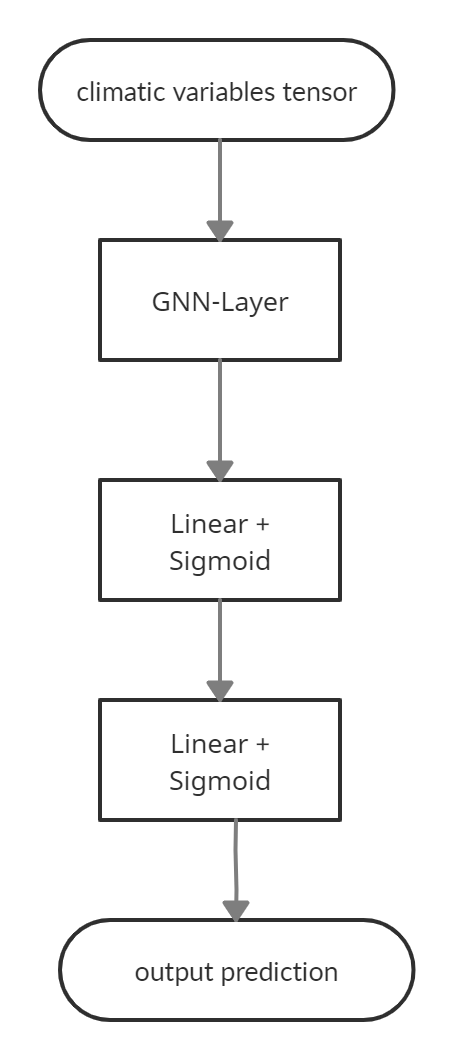
\includegraphics[scale=0.19]{figures/HailNet architecture.png} \\ Resulting architecture
\end{center}

%\subsection{Loss}
%Due to extremeness of hail events, we use Extreme Value Loss \cite{10.1145/3292500.3330896} for classification problem. EVL is similar to Binary Cross Entropy Loss, but EVL penalizes more for mistakes in classification positive (extreme) class.


\section{Computational Experiment}
The experiment goal is to train and evaluate our model on TerraClimate and meteo.ru data.

At every timestamp we have tensor of climatic variables.   
\begin{figure}[h]
\begin{minipage}[h]{0.55\linewidth}
\center{\includegraphics[scale=0.45]{figures/snowmelt_00_2021-05-26.png} \\ snowmelt variable}
\end{minipage}
\hfill
\begin{minipage}[h]{0.55\linewidth}
\center{\includegraphics[scale=0.45]{figures/runoff_00_2021-05-26.png} \\ runoff variable}
\end{minipage}
\end{figure}

These variables corresponds to Krasnodar region.

Using convolution and dense layers it is possible to connect different variables and their spatial neighbourhood. Each hourly climatic tensor transforms to a vector after applying dense and convolution layers and then concatenating outputs from them. After that we have vectors that corresponds to its hour. Until this moment we have just used spatial component of the data. To take in account the temporal component of the data we use LSTM layers to analyze temporal patterns which are typical for hail days.

%\begin{figure}[h]
%\center{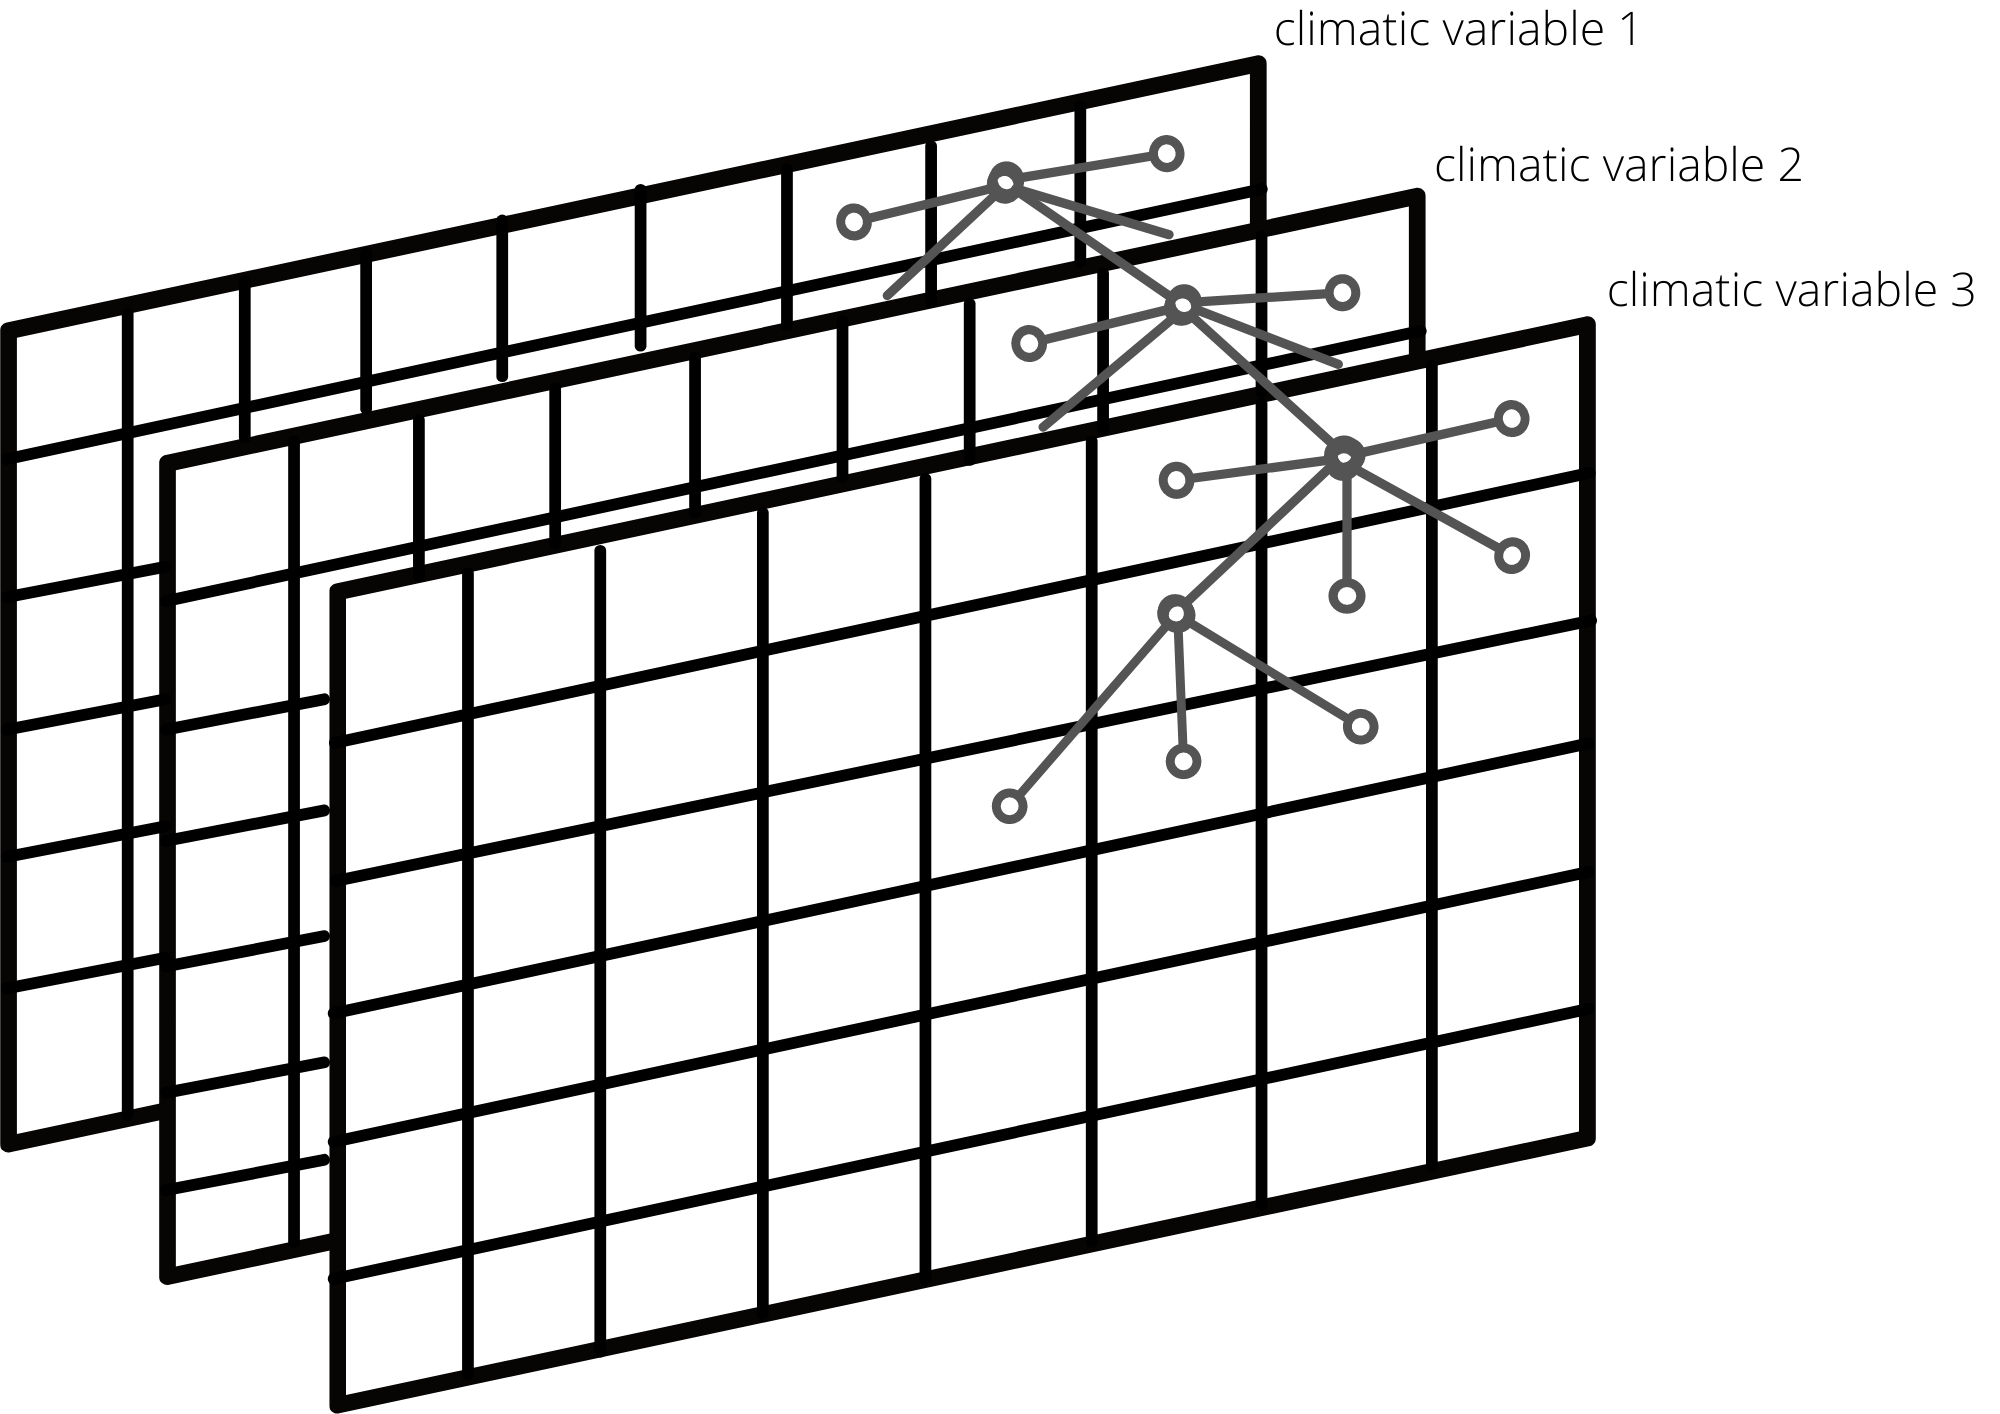
\includegraphics[scale=0.35]{figures/climate variable 1 (1).png} \\ Visualisation of principle}
%\end{figure}



\subsection{Architecture}
HailNet architecture is visualized as following:
\begin{figure}[h]
\center{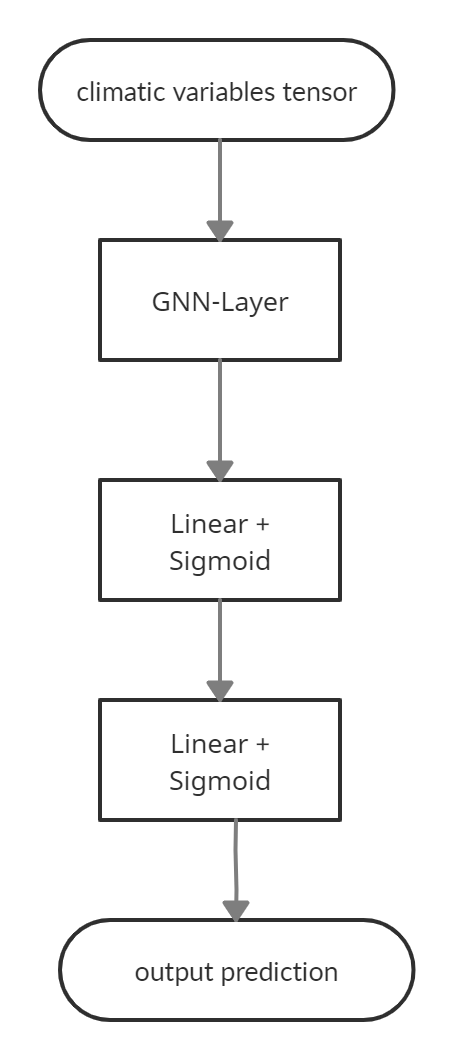
\includegraphics[scale=0.25]{figures/HailNet architecture.png} \\ HailNet architecture}
\end{figure}
\newpage
%In the GNN layer we applying adjacency matrix to climatic tensor to make attention of spatial neighbourhood. After that we applying two linear layers with sigmoid activation function:
%\begin{equation}
%    H_1 = WAX
%\end{equation}
%\begin{equation}
%    H_2 = \sigma(WH_1)
%\end{equation}
%\begin{equation}
%    H_3 = \sigma(WH_2)
%\end{equation}

\subsection{Experiment flow}
\begin{enumerate}
    \item  Creating torch.DataLoader of downloaded climatic data from TerraClimate using Google Earth Engine and hail events data from meteo.ru.
    \item Feed 4-sized batches into training algorithm for 100 epochs.
    \item Updating HailNet parameters optimizing Extreme Value Loss with Adam optimizer.
\end{enumerate}

\section{Error analysis}
Using 22 samples for training we achieve some good c
\center{\includegraphics[scale = 0.7]{figures/trainClassReport.png}\\Training classification report}
\center{\includegraphics[scale = 0.7]{figures/testClassReport.png}\\Testing classification report}


Looking forward to optimize hyperparameters and solve the problem of extreme event classification.
% \section{Preliminary report}
% In order to show how does SMOTE works, there is some experiments with baseline SMOTE + logistic regression on synthetic data . Firstly, created synthetic data for classification problem with imbalanced classes in proportions $98/2$.

% \begin{figure}[h]
% \begin{minipage}[h]{0.49\linewidth}
% \center{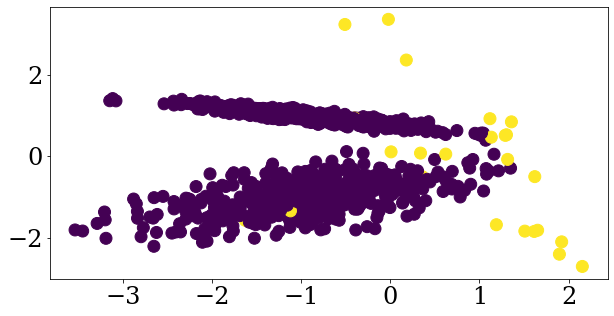
\includegraphics[scale=0.35]{synth_data_before_smote.png} \\ Data distribution before SMOTE}
% \end{minipage}
% \hfill
% \begin{minipage}[h]{0.49\linewidth}
% \center{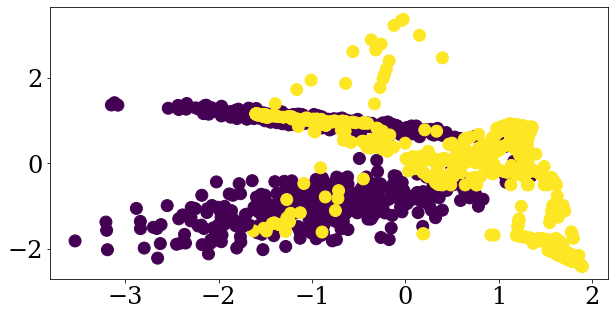
\includegraphics[scale=0.35]{synth_data_after_smote.png} \\ Data distribution after SMOTE}
% \end{minipage}
% \end{figure}

% SMOTE works by selecting examples that are close in the feature space, drawing a line between the examples in the feature space and drawing a new sample at a point along that line. 

% \begin{figure}[h]
% \begin{minipage}[h]{0.49\linewidth}
% \center{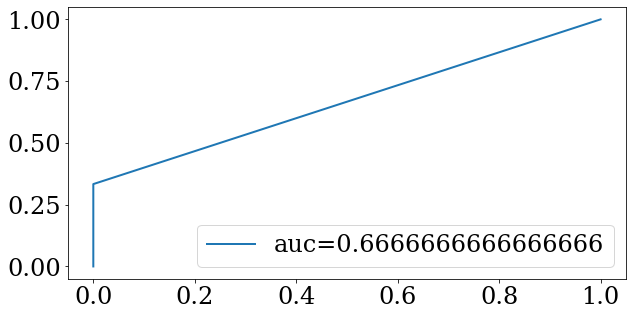
\includegraphics[scale=0.35]{auc_before_smote.png} \\ ROC-curve distribution before SMOTE}
% \end{minipage}
% \hfill
% \begin{minipage}[h]{0.49\linewidth}
% \center{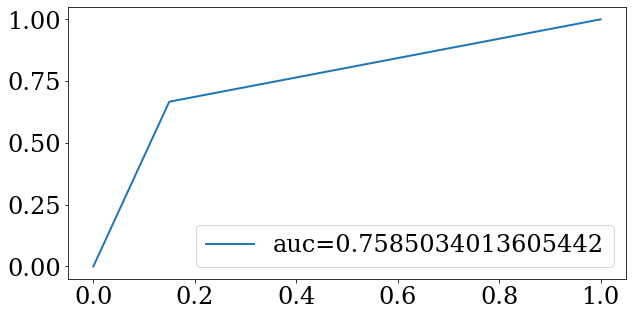
\includegraphics[scale=0.35]{auc_after_smote.png} \\ ROC-curve distribution after SMOTE}
% \end{minipage}
% \end{figure}

% ROC-AUC increased. So we consider that SMOTE make our model better in some cases.

% \section{Baselines}
% The hail risk prediction is classification problems with imbalanced classes. Hail is extreme climatic event. Using SMOTE we can synthesize new examples for the minority classes \cite{DBLP:journals/corr/abs-1106-1813}. SMOTE with logistic regression is our simplest model. This model we use to compare quality with complex one. Logistic regression maps feature space into 1d probability simplex. $\mathbb{R}^n \rightarrow [0,1]$. Logistic regression model is following:
% \begin{equation}
%     y_i = \frac{1}{1 + e^{-x_iw}}
% \end{equation}
% where $x_i$ is feature vector, $w$ is parameters of the model, $y_i$ is probability of positive class labeled "1". $w$ find by LBFGS optimization algorithm minimizing log-loss function. The LBFGS optimization algorithm reviewed in details here \cite{mokhtari2014global}.

    
\newpage
\bibliographystyle{abbrv}

\bibliography{references}

\end{document}